\input{preamble.tex}

\begin{document}


\begin{titlepage}
    \begin{center}
        
        {\Huge \textbf{msave}}
  
        \normalsize
        \vspace{0.5 cm}

        \vspace{0.5cm}
        \begin{centering}
        \hrule
        \vspace{.2cm}
         \LARGE \textbf{A cross-browser extension for saving media}\\

        \end{centering}
        \vspace{1cm}
        

    \end{center}
  \end{titlepage}
  
  %\section*{Abstract}
  %This is an abstract detailing the reason for the project, what was performed and the results of the project.
  
  \newpage
  \tableofcontents
  \newpage
  
  \AddEverypageHook{\Lpagenumber}%
  \cfoot{Page \thepage \hspace{1pt} of \pageref{LastPage}}
  \pagenumbering{arabic} % 
  
  

\section{Introduction}
This report details the development of msave, a cross-browser extension designed to easily save music and media with appropriate metadata from various sites.
Often when listening to music or watching videos online, users want to save the media to their local machine for later use. 

However the process of saving media is often tedious and time consuming, requiring users to manually download the media 
and later modify the metadata to relevant information. 

This tool aims to simplify the process of saving media by creating a process through which 
users can easily save media and describe its metadata while in the browser.
Other features of the tool might include the ability to save media to a playlist, and similar operations.




\section{Planning} \label{sec:planning}
In this section the planning of the project will be documented. 
This includes the project plan, the user stories and the requirements.

\subsection{User stories}
User stories have also been defined for the project. These, including the format of the user stories, are listed below.
\\
\\
\textit{As [who] [when] [where], I [want] because [why].} 
\\
\begin{itemize}
    \item When I am browsing a website, I want to be able to save some media to my music library so that I can listen to it later.
    \item When I am browsing a website, I want to be able to add some media to a playlist so that I can listen to it later.
    \item When I am browsing a website, I want to be able to remove some media from a playlist so that I can remove unwanted media.
    \item When I am saving some media, I want to be able to view whether some media has been saved so that I can avoid adding it twice.
    \item When I am saving some media, I want to be able to add metadata to it so that I can easily identify it later.
    \item When I am browsing a website, I want to be able to view the metadata of some media so that I can verify it is correct.
\end{itemize}

\subsection{Requirements}
In the first iteration of the project, the focus will be on the ability 
to save music from YouTube to a local music library with appropriate metadata.

\subsection*{Functional Requirements}
Table \ref{tab:frequirements} lists the functional requirements for the project.
These requirements are based on the user stories defined in section \ref{sec:planning}.
\begin{table}[H]
\caption{Functional requirements}
%\begin{adjustbox}{width=0.5\textwidth}    % Use if table is too wide
\centering
\begin{tabular}{|l|l|l|}
\hline

\textbf{ID}  & \textbf{Title}                                              & \textbf{MoSCoW} \\ \hline
F1           & Save media to a library from YouTube                        & M               \\ \hline
F1.1         & Save media from YouTube                                     & M               \\ \hline
F1.2         & Configure metadata for the saved media                      & S               \\ \hline
F2           & Display whether the media, or a duplicate, has been saved   & C               \\ \hline
F3           & Remove previously saved media                               & C               \\ \hline
F4           & Add saved media to a playlist                               & C               \\ \hline
\end{tabular}
%\end{adjustbox}  
\label{tab:frequirements}
\end{table}


\subsection*{Non-functional requirements}
Table \ref{tab:nfrequirements} lists the non-functional requirements for the project.
These requirements are based on the user stories defined in section \ref{sec:planning}.

\begin{table}[H]
\caption{Non-functional requirements}
\centering
\begin{tabular}{|l|l|l|}
\hline
\textbf{ID}  & \textbf{Title}                                              & \textbf{MoSCoW}  \\ \hline
NF1          & It should be possible to save music to any music library    & M                \\ \hline
NF2          & It should have a dark mode                                  & C                \\ \hline
NF3          & It must be cross-browser                                    & M                \\ \hline
NF3.1        & It must be support firefox                                  & M                \\ \hline
NF3.2        & It must be support chromium                                 & M                \\ \hline
\end{tabular}
\label{tab:nfrequirements}
\end{table}



\section{Design}
In this section the design of the project will be documented.

\subsection{User Interface}
In this section a mockup of the user interface for the project is detailed.

The image in figure \ref{fig:ui-mockup-1} shows the user interface 
when the user is browsing a website that does not allow the extension to save media.
In the the figure, two buttons can be seen in the top bar.
These buttons are used to check the logs of the extension, and to open the settings page.
The logs tab might be needed to handle errors when saving media.
\begin{figure}[H]
    \centering
    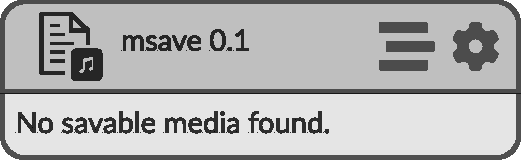
\includegraphics[page=1]{resources/mockup-v0.1.pdf}
    \caption{User interface mockup; no content found.}
\label{fig:ui-mockup-1}
\end{figure}


The image in figure \ref{fig:ui-mockup-2} shows the user interface 
when the user is browsing a website that allows the extension to save media.
The user should be able to select a template or tag that will define 
what type of metadata will be saved with the media.
\begin{figure}[H]
    \centering
    \includegraphics[page=3]{resources/mockup-v0.1.pdf}
    \caption{User interface mockup; no content found.}
\label{fig:ui-mockup-2}
\end{figure}



The image in figure \ref{fig:ui-mockup-3} shows the user interface 
when the user is in the process of saving media.
The fields in the form ought to be configurable in the settings page and relate to templates or tags previously described.
Moreover, some fields should be filled in automatically and others that may have multiple values, such as artists and genres, 
should be written in the same textbox separated by commas.
\begin{figure}[H]
    \centering
    \includegraphics[page=4]{resources/mockup-v0.1.pdf}
    \caption{User interface mockup; no content found.}
\label{fig:ui-mockup-3}
\end{figure}



\subsection{Components}
WIP

\subsubsection{Interfaces}
WIP





\section{Implementation}
WIP

\subsection{Selection sort}
WIP


\section{Discussion}
WIP

\section{Conclusion}
WIP


%\printbibliography

%\appendix
%\section*{\appendixname}
%\addcontentsline{toc}{section}{\appendixname}
%\renewcommand{\thesubsection}{\Alph{subsection}}
%

%\subsection{Diagram} \label{common}
%\begin{figure}[H]
%    \centering
%    \includegraphics[width=\textwidth]{image.png}
%    \caption{Caption}
%\end{figure}

%\subsection{Pdf file to include}
%\includepdf[pages=-,pagecommand={},width=\textwidth]{file.pdf}



\end{document}